%----------------------------------------------------------------------------------------------------------------------

\begin{frame}{Proposed Idea}

\begin{itemize}[noitemsep,label=\textbullet,topsep=2pt,parsep=2pt,partopsep=2pt]
\item Use of Feature Tree
\item The model feature tree is traversed and candidate features for suppression are identified based on a set of criteria. 
\item Rules specific to Sheet Metal Features. Features like emboss, spot, weld, hem, relief, louver etc. These, by their own definition, are sort-of helpers/secondary features. They are not part of main Shape. So they are suppressed
\item Face-Cluster method for remaining-generic features
\end{itemize}
\end{frame}

%----------------------------------------------------------------------------------------------------------------------

\begin{frame}{Algorithm  First pass - Sheet Metal specific}

	\begin{itemize}[noitemsep,label=\textbullet,topsep=2pt,parsep=2pt,partopsep=2pt]
	\item From bottom, go upwards till Unfold features are suppressed
	\item Based on Sheet Metal feature type, criticality add to suppression
	\item Regenerate model by excluding the features in suppression
	\end{itemize}
\end{frame}

\begin{frame}{Algorithm Second pass - generic}

	\begin{itemize}[noitemsep,label=\textbullet,topsep=2pt,parsep=2pt,partopsep=2pt]
		\item {\bf Size criterion}: Get either Part's Bounding Box ({\bf pBB}), it's diagonal length or summation of area of faces, and based on a threshold (say, 5\%). calculate the threshold size {\bf D} below which a feature(set) is considered  'small'
		\item {\bf Final Body}: Iterate over final body faces, not finding (full tool-body) feature's parameters. 
		\item {\bf Reason}: some of the features get engulfed fully or partially during the forward-create.
		\item {\bf Remnant Face}: For each remnant face, get its owning feature. Build a table with entries of each Cluster (remnant-faces having same feature owners).
		\item Add each cluster-owning feature to suppression based on the Rules 
		\end{itemize}

The resultant model can then be used for Midsurface generation.

\end{frame}

%----------------------------------------------------------------------------------------------------------------------
\begin{frame}{Autodesk Inventor Sheet Metal has following features}

\begin{table}[!h]
\begin{tabular}[h]{@{}l l l l @{}}

\textcolor{yellow}{AliasFreeForm}	&
\textcolor{green}{Bend} &
\textcolor{green}{BendPart} &
\textcolor{blue}{Boss} \\

\textcolor{yellow}{BoundaryPatch} &
\textcolor{blue}{Chamfer} &
\textcolor{cyan}{CircularPattern} &
\textcolor{cyan}{Client} \\

\textcolor{blue}{Coil} &
\textcolor{blue}{Combine} &
\textcolor{green}{ContourFlange} &
\textcolor{green}{ContourRoll} \\

\textcolor{green}{CoreCavity} &
\textcolor{green}{CornerChamfer} &
\textcolor{green}{Corner} &
\textcolor{green}{CornerRound} \\

\textcolor{blue}{Cut} &
\textcolor{cyan}{Decal} &
\textcolor{blue}{Deleteface} &
\textcolor{blue}{Emboss} \\

\textcolor{yellow}{Extend} &
\textcolor{blue}{Extrude} &
\textcolor{blue}{FaceDraft} &
\textcolor{green}{Face} \\

\textcolor{blue}{FaceOffset} &
\textcolor{blue}{Fillet} &
\textcolor{green}{Flange} &
\textcolor{green}{Fold} \\

\textcolor{green}{Grill} &
\textcolor{green}{Hem} &
\textcolor{blue}{Hole} &
\textcolor{green}{Knit} \\

\textcolor{green}{Lip} &
\textcolor{green}{LoftedFlage} &
\textcolor{blue}{Loft} &
\textcolor{yellow}{Midsurface} \\

\textcolor{cyan}{Mirror} &
\textcolor{blue}{MoveFace} &
\textcolor{cyan}{Move} &
\textcolor{cyan}{NonParametricBase} \\

\textcolor{green}{PunchTool} &
\textcolor{cyan}{RectangularPattern} &
\textcolor{green}{Refold} &
\textcolor{blue}{ReplaceFace} \\

\textcolor{green}{Rest} &
\textcolor{blue}{Revolve} &
\textcolor{green}{Rib} &
\textcolor{green}{Rip} \\

\textcolor{blue}{RuleFillet} &
\textcolor{blue}{Sculpt} &
\textcolor{blue}{Shell} &
\textcolor{green}{SnapFit} \\

\textcolor{cyan}{Split} &
\textcolor{blue}{Sweep} &
\textcolor{yellow}{Thicken} &
\textcolor{blue}{Thread} \\

&\textcolor{cyan}{Trim} &
\textcolor{green}{Unfold} &\\
\\
\textcolor{yellow}{Surface} &
\textcolor{blue}{Solid} &
\textcolor{green}{SheetMetal} &
\textcolor{cyan}{Others}\\

\end{tabular}
\end{table}
%----------------------------------------------------------------------------------------------------------------------

\end{frame}

%--------------------------------------------------------------------------------------------------------------
\begin{frame}{Sheet Metal features which are not critical to Principal Shape}
\begin{tabular}[h]{@{} p{0.45\linewidth} p{0.45\linewidth}@{}}

CornerRelief

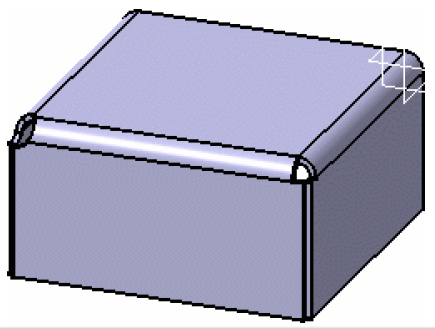
\includegraphics[width=0.8\linewidth]{..//Common/images/Feature_CornerRelief.png} &

Louver

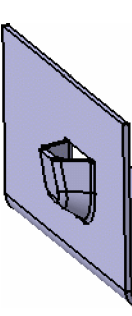
\includegraphics[width=0.3\linewidth]{..//Common/images/Feature_Louver.png} \\

Bridge

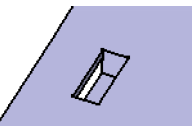
\includegraphics[width=0.8\linewidth]{..//Common/images/Feature_Bridge.png} &

Hem


\includegraphics[width=0.4\linewidth]{..//Common/images/Feature_Hem.png} \\

\end{tabular}
\end{frame}
%----------------------------------------------------------------------------------------------------------------

%--------------------------------------------------------------------------------------------------------------
\begin{frame}{Sheet Metal features which are grouped together}
\begin{tabular}[h]{@{} p{0.6\linewidth}@{}}

Mirror

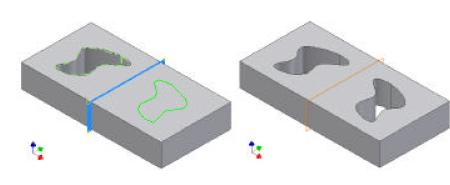
\includegraphics[width=0.6\linewidth]{..//Common/images/Feature_Mirror.png} \\

Circular Pattern

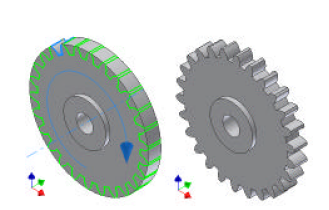
\includegraphics[width=0.6\linewidth]{..//Common/images/Feature_CircPattern.png} \\

Rectangular Pattern

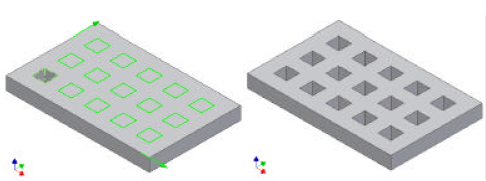
\includegraphics[width=0.6\linewidth]{..//Common/images/Feature_RectPattern.png} \\

Grill \\

\end{tabular}

\end{frame}
%--------------------------------------------------------------------------------------------------------------
\begin{frame}{Sheet Metal features which are left for Remnant Face Logic}
\begin{tabular}[h]{@{} p{0.3\linewidth} p{0.3\linewidth} p{0.3\linewidth}@{}}

Face-Wall

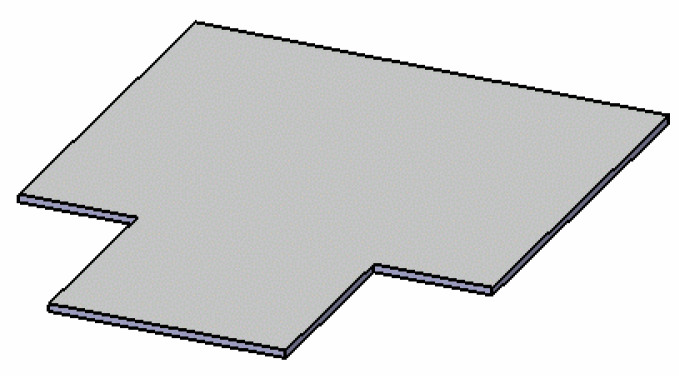
\includegraphics[width=0.9\linewidth]{..//Common/images/Feature_Wall.png} &

Bend


\includegraphics[width=0.6\linewidth]{..//Common/images/Feature_Bend.png} &

Flange

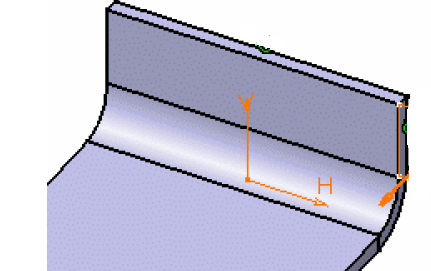
\includegraphics[width=0.9\linewidth]{..//Common/images/Feature_Flange.png} \\

Stamping

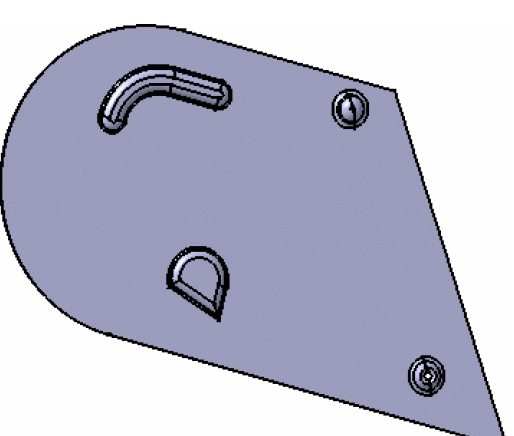
\includegraphics[width=0.9\linewidth]{..//Common/images/Feature_Stamping.png} &

Cutout

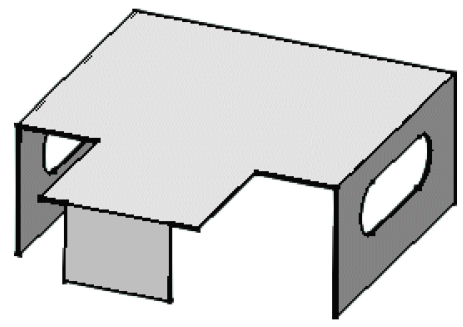
\includegraphics[width=0.6\linewidth]{..//Common/images/Feature_Cutout.png} &

Rib

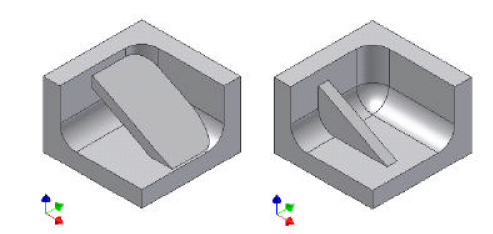
\includegraphics[width=0.9\linewidth]{..//Common/images/Feature_Rib.png} \\

\end{tabular}
\end{frame}
%----------------------------------------------------------------------------------------------------------------

\begin{frame}{Remnant Face Logic}

\begin{itemize}[noitemsep,label=\textbullet,topsep=2pt,parsep=2pt,partopsep=2pt]
\item Some of the features get engulfed fully or partially
\item Decision-to-suppress on the relative size of remnant feature-faces and NOT on the original size of the feature faces

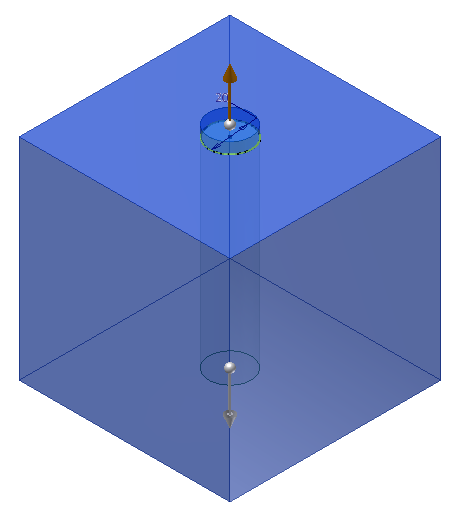
\includegraphics[width=0.2\linewidth]{..//Common/images/Solid_Simple_SmallProtrusion.png}
\item For each remnant face, get its owning feature. 
\item Build a table with entries of each Cluster
\vskip 2mm
\begin{tabular}[h]{@{} p{0.3\linewidth} p{0.3\linewidth}@{}p{0.3\linewidth} }
\textbf{Face ID} & \textbf{Size Criterion} & \textbf{Owning Feature}\\
$f_1, f_4, f_5$ &	0.25	& Extrude1\\
$f_6, f_2, f_3, f_7, f_8$	& 0.12	& Hole2\\
$f_9, f_{11}$	& 0.25	& Extrude15\\
$f_{10}, f_{12}, f_{15}, f_{14}$ &	0.54	& Hole21\\
\end{tabular}
\end{itemize}

\end{frame}
